\documentclass{llncs}

\usepackage{bookmark}
\usepackage{nth}
\usepackage{cite}
\usepackage{enumerate} 
\usepackage{subfig}
\usepackage{graphicx}
\usepackage{mwe}
\usepackage{rotating}
\usepackage{colortbl}
\usepackage{array}
\usepackage{subfig}
\usepackage{fixltx2e}
\usepackage[latin9]{inputenc} 
\usepackage{listings}
\usepackage{tabularx}
\usepackage{multirow}
\usepackage[table]{xcolor}


\usepackage{fmtcount}
\usepackage{booktabs,caption,fixltx2e}
\usepackage[flushleft]{threeparttable}
\begin{document}


\title{A Systematic Review on Architecture-Driven Modernization}

\author{Rafael Durelli, Bruno}

\institute{Lab, University, Address}
\maketitle

\begin{abstract}

\underline{\textbf{Background:}} Architecture-Driven Modernization (ADM) has become a popular approach for modernizing legacy systems by means of Model-Driven Development (MDD). It uses standard and language independent metamodels, such as Knowledge Discovery Metamodel (KDM). The whole process involves reverse engineering a system into a KDM instance, refactoring it obtaining a modernized KDM and generating the modernized system. Although the interest in ADM has grown in the last years, to the best of our knowledge, there is neither published systematic review nor survey which presents the current state of the art and research directions in this field. Therefore, we claim that there is a need for evidence-based body of knowledge about different aspects of the adoption of ADM. \underline{\textbf{Objective:}} Presenting a systematic review that exposes the current state of the art and research directions in the ADM field. \underline{\textbf{Method:}} A systematic review on ADM was performed using Kitchenham's guidelines which consist of three main phases: (\textit{i}) planning, (\textit{ii}) conducting and (\textit{iii}) reporting. \underline{\textbf{Results and conclusion:}} Classification schemes have been defined and the 30 primary studies have been selected and classified on the basis of focus area, contribution type and research type. Four focus area have been identified. Papers that illustrated process and tools to assist the modernization of legacy system by means of ADM are in a majority. The majority of research type are evaluation research. We claim that the findings of this paper provide interesting insights into different aspects of ADM. Also, we expect that the findings can provide valuable information to readers on what can be expected from applying ADM and its metamodels to modernize legacy systems. Furthermore, the results can provide perception of new research in the modernization area for investigating and defining new tools/process to assist the modernization of legacy systems.

\end{abstract}

\section{Introduction}\label{sec:Introduction}
\linespread{0.87}
Software systems are considered legacy when their maintenance costs are raised to undesirable levels but they are still valuable for organizations. Therefore, they can not be discarded because they incorporate a lot of embodied knowledge due to years of maintenance. As these systems still provide significant business value, they must then be modernized so that their maintenance costs can be manageable and they can keep on assisting in the regular daily activities. 

%The first task that must be performed in order to carrying out a software modernization is understand the legacy system. This is not a trivial task; in fact studies estimate that between $50$ percent and $90$ percent of software maintenance involves developing an understanding of the software being maintained~\cite{Tilley95perspectiveson}, thus several approaches have been developed to support software engineers in the comprehension of systems where reverse engineering (RE) is one of them~\cite{Canfora2011}. RE supports program comprehension by using techniques that explore the source code to find relevant information related to functional and non-functional features~\cite{chikofskyTax}.

In this context, OMG has defined standards in the modernization process, creating the concept of ADM. ADM follows the MDD~\cite{5440163} guidelines and comprises three major steps. Firstly, a reverse engineering is performed starting from the source-code and a model instance Plataform-Specific Model (PSM) is created. Secondly, successive transformations are applied to this model up to reach a good abstraction level in a model called KDM (Knowledge Discovery Metamodel). Upon this model, several modernization, optimizations and modifications can be performed in order to solve problems found in the legacy system. Then, a forward engineering is carried out and the source code of the modernized target system is generated. According to the OMG the most important artifact provided by ADM is the KDM metamodel, which is a multipurpose standard metamodel that represents all aspects of the existing IT (Information  Technology) architectures. The idea behind the standard KDM is that the community starts to create parsers from different languages to KDM. As a result everything that takes KDM as input can be considered platform and language-independent. For example, a refactoring catalogue for KDM can be used for refactoring systems implemented in different languages. 

In order to  present the current state of the art and research directions in this field, we performed a systematic review of ADM and its metamodels. Our motivation to realize a systematic review is to identify areas that have been studied and conducted related to ADM and its metamodels. Although, ADM is relatively a recent approach, OMG claims that it is a standardization that aiming to join two known research field, (\textit{i}) Model-Driven Development and (\textit{ii})Software Reengineering. Thus, we argue that identifying possible gaps that have not been researched and presenting results from literature are valuable from perspective of possible future enhancements and use.  Although several studies have been reported in the context of ADM~\cite{PerezCastillo20121370, SMR:SMR582, FuentesFernandez2012247, PrezCastillo2011519}, to the best of our knowledge none systematic review has been conducted in the field of ADM and its metamodels. As for the fact that various types of research have appeared addressing diversifying focus areas related to the topic of modernization of legacy system by means of ADM, we claim the need for a more systematic investigation of this topic. Also we argue that this paper can help researchers in the field of modernization of legacy systems, once it provides an overview of the current state-of-the-art of the ADM. Furthermore, it serves as a first step towards more thorough examination of the topics addressed in it with the help of systematic literature reviews.

% If we consider Software Reengineering and Model Driven Development, the ADM approach, advocated by the OMG, is relatively recent and its first official records date is of 2003. However, ADM is a recent approach OMG claims that it is a standarlization to join Model Driven Development and Software Reengineering. Therefore, we argue that  identifying possible gaps that have not been met by ADM and try to use the works found as a reference for works of the researchers involved in this article are also objectives of this paper.



%This study also aims at identifying and presenting results from literature that are valuable from perspective of possible future enhancements and use. Although several studies have been reported in the context of ADM~\cite{PerezCastillo20121370, SMR:SMR582, FuentesFernandez2012247, PrezCastillo2011519}, to the best of our knowledge none systematic review has been conducted in the field of ADM and its metamodels. As for the fact that various types of research have appeared addressing diversifying focus areas related to the topic of modernization of legacy system by means of ADM, we claim the need for a more systematic investigation of this topic. Thus, this paper aims to present a systematic review describing research into ADM. Also we argue that this paper help researchers in the field of modernization of legacy systems, once it provides an overview of the current state-of-the-art of the ADM. Furthermore, it serves as a first step towards more thorough examination of the topics addressed in it with the help of systematic literature reviews.

Following this introduction, this paper is structured as follows: In Section~\ref{method}, describes how the systematic review methodology has been planned, conducted and reported. In Section~\ref{sec:discussion_and_threats} there are the principle findings and the threats to validity of this study. Concluding remarks are made in Section~\ref{conclusion}.

\section{The Systematic Review}\label{method}

This study was undertaken as a systematic review based on the guidelines proposed by Kitchenham and Brereton~\cite{Kitchenham} which consist of three main phases: (\textit{i}) planning, (\textit{ii}) conducting and (\textit{iii}) reporting. %In Figure~\ref{process_systematic_review} depicts these three phases that we carried out herein. 
%Furthermore, in this paper we have used Visual Text Mining (VTM) technique to support the studies selection~\cite{Malheiros:2007}. VTM uses text mining algorithms and methods combined with interactive visualisations. Therefore, it can help the user making sense of a collection of primary studies, without actually reading all of them. In this case the studies were reading partially or full. The following sections present details on how each phase was carried out.

%\begin{figure}[!h]
%\centering
  % Requires \usepackage{graphicx}
%  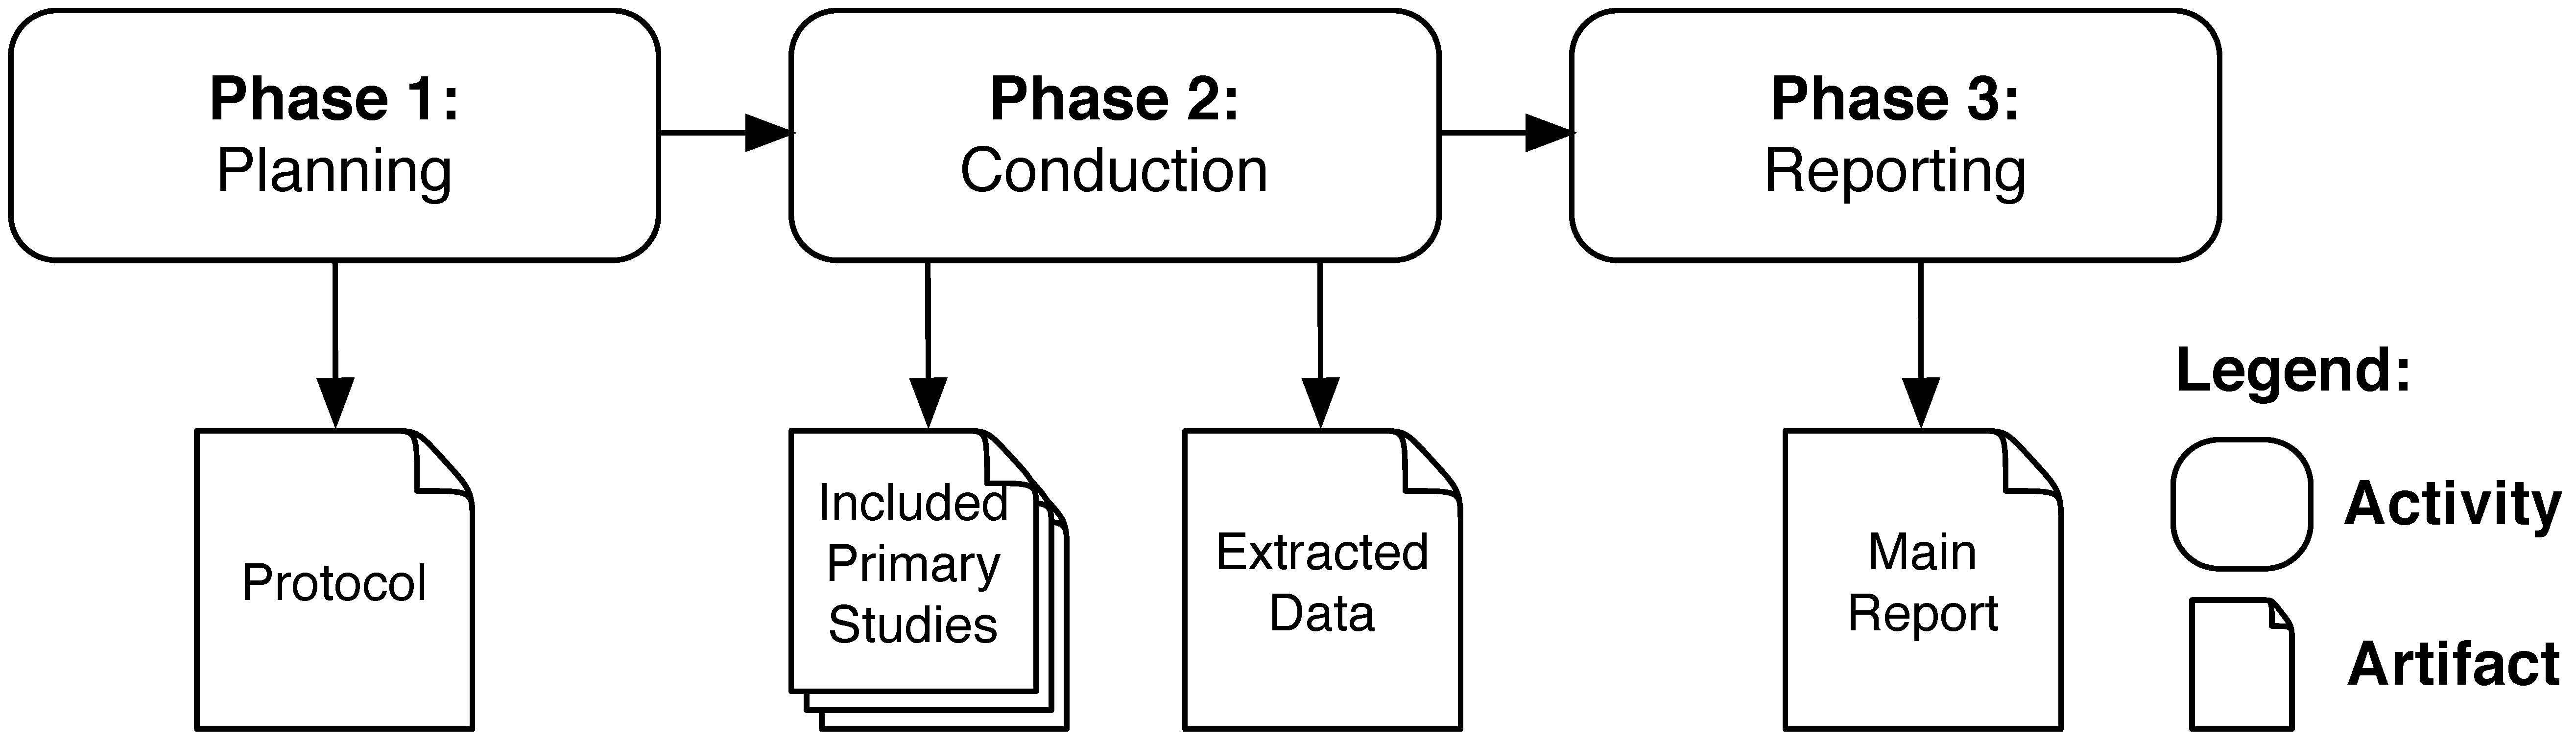
\includegraphics[scale=0.09]{figuras/process}
%\caption{Systematic review process (Adapted from Kitchenham~\cite{Kitchenham}).}
%\label{process_systematic_review}
%\end{figure} 
	\subsection{Planning the Systematic Review}\label{planning}
	In this phase we defined the review protocol. This protocol contains: (\textit{i}) the research questions, (\textit{ii}) the search strategy, (\textit{iii}) the inclusion and exclusion criteria and (\textit{iv}) the data extraction and synthesis method.

%Research questions must embody the review study purpose. Moreover, these questions reflect the general scope of the review study. The scope is comprised of population (i.e., population group observed by the intervention), intervention (i.e., what is going to be observed in the context of the planned review study), and outcomes of relevance (i.e., the results of the intervention). Furthermore, during the conduction of this step, it was also necessary to establish the scope of the review study. According to the systematic review process~\cite{Kitchenham}, the scope has to be established using the PICO criteria. Thus, herein our \textbf{Population} is published scientific literature reporting on the use of Architecture-Driven Modernization and its metamodels. The \textbf{Intervention} is published scientific literature interested with Architecture-Driven Modernization and its metamodels. The \textbf{Comparison} is not applied herein. Finally, the \textbf{Outcomes of relevance} is an overview of the studies that have been conducted in the field of Architecture-Driven Modernization and its metamodels, emphasizing primary studies that report on the process used in the research area, from observing such an aggregated data set, we also intend to provide insight into the frequencies of publication over time to inspect trends.   

%\begin{itemize}

%\item \textbf{Population:} published scientific literature reporting on some existing mining techniques for crosscutting concern.

%\item \textbf{Intervention:} published scientific literature concerned with mining techniques for crosscutting concern. Furthermore, we also aim at determining which techniques are the most used within academic settings.

%\item \textbf{Comparison:} No applied herein.

%\item \textbf{Outcomes of relevance:} an overview of the studies that have been conducted in the field of crosscutting concern mining, emphasizing primary studies that report on the techniques used in the research area. From observing such an aggregated data set we also intend to provide insight into the frequencies of publication over time to inspect trends.

%\end{itemize} 

%Como ADM esta sendo aplicada na literatura para auxiliar a modernizacao de sistemas legados

The objective of this review is to find out \textbf{how ADM has been applied in the literature to assist engineers during the process of modernization of legacy systems}. In order to achieve such objective we formulated three research questions, as can be seen in Table~\ref{tab:research_questions}.

\begin{table}
\centering
\caption{Research questions\label{tab:research_questions}}
\begin{tabularx}{
1.0\textwidth}{|c|X|X|}
\hline 
RQ$_1$: & What are the focus areas most discussed and least discussed in the
literature regarding the ADM? Moreover, what types of contributions
have been presented so far?\tabularnewline
\hline 
RQ$_2$: & Given the ADM's standards metamodels, which one has been more used
in the literature? In addition, given the identified metamodel, what
are the packages most and least used?\tabularnewline
\hline 
RQ$_3$: & Which research types have been employed into the field herein?\tabularnewline
\hline 
\end{tabularx}
\end{table}

% \textbf{RQ$_1$:} What are the focus areas most discussed and least discussed in the literature regarding the ADM? Moreover, what types of contributions have been presented so far?; \textbf{RQ$_2$:} Given the ADM's standards metamodels, which one has been more used in the literature? In addition, given the identified metamodel, what are the packages most and least used?; \textbf{RQ$_3$:} Which research types have been employed into the field herein?;% \textbf{RQ$_4$:} Which are the existing tools support for ADM? Moreover, how do the tools perform the identification of what needs to be modernized?

%\begin{description}

%\item[\textbf{RQ$_1$:}] What are the focus area most discussed and least discussed in the literature regarding the ADM? Moreover, what types of contributions have been presented so far?

%\item[\textbf{RQ$_2$:}] Given the ADM's standards metamodels, which one has been more used in the literature? In addition, given the identified metamodel, what are the packages most and least used?

%\item[\textbf{RQ$_3$:}] Which research types have been employed into the field herein?

%\item[\textbf{RQ$_4$:}] Which avenues are often used to publish research related to ADM?

%\item[\textbf{RQ$_5$:}] Which are the existing tool support for ADM? Moreover, how the tools perform the identification of what needs to be modernized?

%\item[\textbf{RQ$_4$:}] Given a set of concerns, which are the most indicated techniques for performing the mining?

%\item[\textbf{RQ$_5$:}] How can someone combine the techniques for improving the precision and recall metrics?

%\item[\textbf{RQ$_3$:}]  Considering the techniques that we found, which ones have automated support?

%\end{description}

To address \textbf{RQ$_1$}, all the primary studies picked during the the selection stage were  read in order to identify the focus area of each study. Next, we arrange all studies according to the focus area. Whether any kind of disagreement related to the focus area that the article meets, it was marked and was discussed with everyone involved in the review in order to clarify which topic it belongs. With respect to \textbf{RQ$_2$}, we also read all primary studies and identified which metamodel was used in the study. Finally, with respect to \textbf{RQ$_3$}, we used and adapted the scheme proposed by Wieringa et al.,~\cite{Wieringa:2005:REP:1107677.1107683} in order to classify each primary study into a research type. %Finally, to address \textbf{RQ$_4$} we read all primary studies in order to identify the tools used to modernize the legacy systems. %Next, we arrange the identified tools according to the focus area. 


Afterwards, we defined the search string and chose the electronic databases. The search string was created based upon a set of keywords. Figure~\ref{search_string} shows the search string elaborated. 

\begin{figure}[!h]
\centering
  % Requires \usepackage{graphicx}
  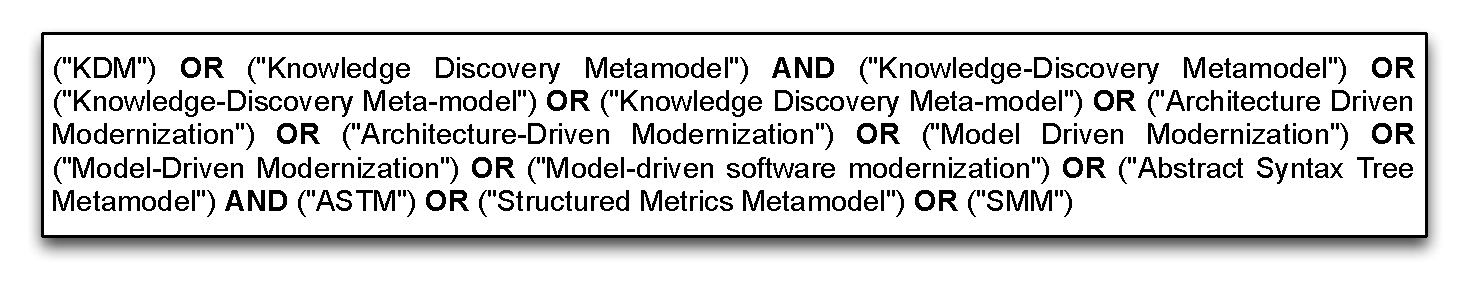
\includegraphics[scale=0.35]{figuras/SearchStringADM}
\caption{Search String.}
\label{search_string}
\end{figure} 

The search encompassed electronic databases which are deemed as the most relevant scientific sources~\cite{Kitchenham} and therefore likely to contain important primary studies. We used the search string on the following electronic databases: \textit{ACM}, \textit{IEEE XPLORE}, \textit{Scopus}, \textit{Web of Science} and \textit{Engeneering Village}. Note that since the features provided by various databases, as well as the exact syntax of search strings to be applied vary from one database to other, the string given in Figure~\ref{search_string} was actually used to construct a semantically equivalent string specific to each database. Furthermore, no limits were placed on date of publication with a view to not restrict the review study scope. Aimed at keeping track of the selected papers, we used JabRef\footnote{http://jabref.sourceforge.net/}, an open source system for bibliography reference management. 



In order to determine which primary studies are relevant to answer our research questions, we applied a set of inclusion and exclusion criteria. Inclusion criteria applied were: (\textit{i}) \textbf{The primary study presents at least one solution of modernization by means of ADM} - (\textit{ii}) \textbf{Studies that explicitly present an ADM approach} - (\textit{iii}) \textbf{The primary study presents at least one type of evaluation technique for ADM}. 

%\begin{enumerate}[(i)]%for small alpha-characters within brackets.
%\item \textbf{The primary study presents at least one solution of modernization by means of ADM:} the paper provides evidences that the ADM assists the software engineer during the modernization/refactoring of legacy system.
%\item \textbf{Studies that explicitly present an ADM approach:} the paper provides an approach to assist the software engineer to modernize the legacy system.
%\item \textbf{The primary study presents at least one type of evaluation technique for ADM:} without the results of the evaluation we would not be able to make comparisons desired. In other words, the paper must clearly present which assessment techniques have been employed to evaluate the ADM process, i.e., case study, experiment, survey, etc.
%\end{enumerate}

Not all of these criteria must be present for every primary study. However, at least the former, i.e., (a), must be present. If all criteria were mandatory, the number of selected techniques would decrease significantly.

Exclusion criteria applied were: (\textit{i}) \textbf{Papers which mentioned ADM and its metamodels only in the abstract} - (\textit{ii}) \textbf{Introductory papers for books and workshops} and (\textit{iii}) \textbf{The primary study is a short paper}. We elaborated data extraction forms to accurately record the information obtained by the researchers from the primary studies. The form for data extraction provides some standard information, such as (\textit{i}) a brief of the primary study, highlighting where ADM and its metamodels were used, (\textit{ii}) date of data extraction, (\textit{iii}) title, authors, journal, publication details and (\textit{iv}) a list of each conclusion and statement encountered for each question. During the extraction process, the data of each primary study were independently gathered by all reviewers. 

The review was performed in August, 2013 by three M.Sc., a Ph.D. student and three expert. All the results of the search process are documented in the web material(tinyurl.com/99spmaz). So, it is clear to others how thorough the search was, and how they can find the same documents.

	\subsection{Conducting the Systematic Review}\label{conducting}
	%In Figure 2~\ref{process} the three steps of the conduction phase. As can be seen, in Step 1, we identified primary studies in the digital libraries. The digital libraries Scopus has returned more primary studies than the others(262), i.e., IEEE, ACM and Springer have returned 215, 202 and 127, respectively. Possibly, this came about because this digital library indexes studies of others libraries, such as IEEE and Springer. Summing up, we have gotten 802 primary studies in the Step 1. In the Step 2 we have selected the primary studies by means of reading the titles and abstracts and the application of the inclusion and exclusion criteria. As a result, we have gotten a total of 124 primary studies that were read entirely, so the upshot obtained in the Step 3 were 62. Among these 62 primary studies we have identified 18 mining techniques for crosscutting concern. Therefore, each included primary study was assigned to one or more techniques.
%
%\begin{figure}[!h]
%\centering
%  % Requires \usepackage{graphicx}
%  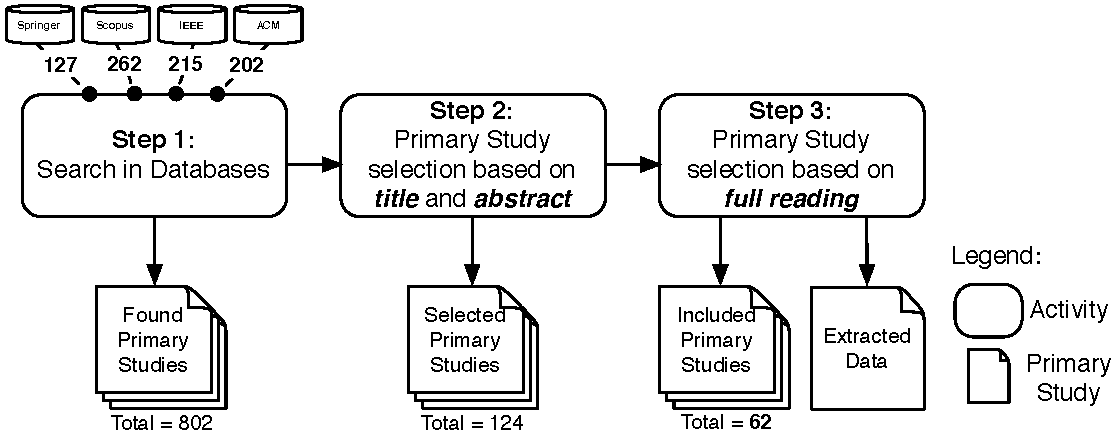
\includegraphics[scale=0.4]{figuras/process_conducted}
%\caption{Papers retrieved from each electronic database, total of candidate studies and the final set.}
%\label{process}
%\end{figure} 

Firstly we applied the search string given in Figure~\ref{search_string} in some digital libraries. An overview of results acquired from these digital libraries is depicted in Table~\ref{result_digital}.
\begin{table}[!h]
\centering
\caption{Overview of search results.}
\begin{tabular}{p{\dimexpr.25\textwidth}p{\dimexpr.16\textwidth-4\tabcolsep}}
\hline 
Digital Libraries & Number\tabularnewline
\hline 
Scopus & 150
\\
ACM & 51
\\ 
Engeneering Village & 30
\\
Web of Science & 17
\\
IEEE & 11
\\
Total & 259
\\
Candidates & 82
\\
Final set & 30\tabularnewline
\hline 
\end{tabular}
\label{result_digital}
\end{table} 
As can be seen in this table, the digital libraries Scopus returned more primary studies than the others (150), ACM, Engeneering Village, Web of Science and IEEE returned 51, 30, 17 and 11, respectively. Possibly, this occurred because Scopus indexes studies of others libraries, such as IEEE and ACM. Summarizing, we obtained 259 primary studies. After performing automatic search, we excluded the duplicate publications. If a primary study was found in more than once, we selected the most recent and detailed version of the paper. Afterwards, we selected the primary studies by reading the titles and abstracts and the application of the inclusion and exclusion criteria. At this stage, we also narrowed down the categories of publications to some extent by excluding non-peer reviewed publications, in order to ensure a level of quality as well as to avoid redundancy in contributions. As a result, we acquired a total of 82 primary studies that were read entirely, so the upshot obtained were 30 studies. A total of 229 studies were excluded either due to their limited relevance or meeting one of the other exclusion criterions.

We applied the classification schemes proposed by Petersen et al.~\cite{Petersen:2008:SMS:2227115.2227123} and classified the publications into categories from three perspectives, as follows: (\textit{i}) focus area, (\textit{ii}) contribution type and (\textit{iii}) research type. We chose this classification scheme because it is highly used in secondary study, i.e., papers which describe systematic review~\cite{Durelli:2013:SRM:2480362.2480567}.% and systematic mapping~\cite{Mehmood:2013:AMC:2400747.2401009}. %Although, this classification schemes has been proposed to be applied during a systematic mapping, we claim that it can be used during the systematic review process as well. 
 Thus, the aforementioned categories were adapted to our systematic study. We identified four focus areas, five contribution types and five research types. Notice that the research types reflects the research approach used in the primary study. We used and adapted the scheme proposed by Wieringa et al~\cite{Wieringa:2005:REP:1107677.1107683} herein. The resultant classification schemes are as follows:

\begin{enumerate}

\item Focus Areas: 

\begin{enumerate}

\item Software Modernization: This focus area is related to primary studies which describe approaches that use ADM to fully modernize legacy systems either to another platform  or architecture;

\item Business Knowledge Extraction: Describes primaries studies which address process, method or approach to extract business process of a legacy system;

\item Concern Extraction: Describes primaries studies which address process, method or approach to extract crosscutting concerns (CC) of a legacy system. Examples of CC are persistence, security and distribution;

\item Extension of ADM's Metamodels: This focus area represents primary studies which report an approach, method or process to extend one of the ADM's metamodels;

\item Applicability: This category includes papers that mainly focus on reporting evidence related to applying ADM and its metamodels in practice. In other words, papers which enable researchers and practitioners to get a better understanding and utilization of ADM and its metamodels.

\end{enumerate}

\item Contribution Type:

\begin{enumerate}

\item Tool: Refers to primary studies that focus on providing tools to support the modernization of legacy system by using ADM; 

\item Process: Refers to papers which describe processes to assist the modernization of legacy system by means of ADM;

\item Model Transformation: Refers papers that describe the use of language transformation such as Query/Views/Transformations (QVT)\footnote{http://www.omg.org/spec/QVT/1.1/} or ATL Transformation Language (ATL)\footnote{www.eclipse.org/atl/} to realize transformation among the ADM's metamodels;

\item Metamodel: Describes primary studies which create or extend the ADM's metamodels to deal with a specific problem, for instance, providing a KDM light-weight extension in order to either represent the aspect oriented paradigm or supports a component-oriented decomposition;

\item Metrics: Describes papers that focus on proposing or applying metrics to effectiveness of ADM and its metamodels.

\end{enumerate}

\item Research Type:

\begin{enumerate}

\item Validation research: Validation research is conducted in a systematic way and may present any of these: prototypes, math analysis, etc;

\item Evaluation research: In contrast to validation research, evaluation research aims at examining a solution that has already been practically applied. It investigates the practical implementation of solution and usually presents results using field studies, experiments, or case studies, etc;

\item Conceptual proposal: A conceptual proposal presents an arrangement to perceive things that already exist, in a novel way;

\item Experience paper: An experience paper reports on personal experience of the author from one or more real life projects;

\item Opinion paper:  Opinion papers report on personal opinion of the author on suitability or unsuitability of a specific technique or tool.

\end{enumerate}

\end{enumerate}
	\subsection{Reporting the Systematic Review}\label{reporting}
	

The focus of this section is to present broad overview of research within ADM after conducting the systematic review. Moreover, we used information drawn from this overview to answer the research questions. 

\begin{figure*}[t]
\centering
  % Requires \usepackage{graphicx}
  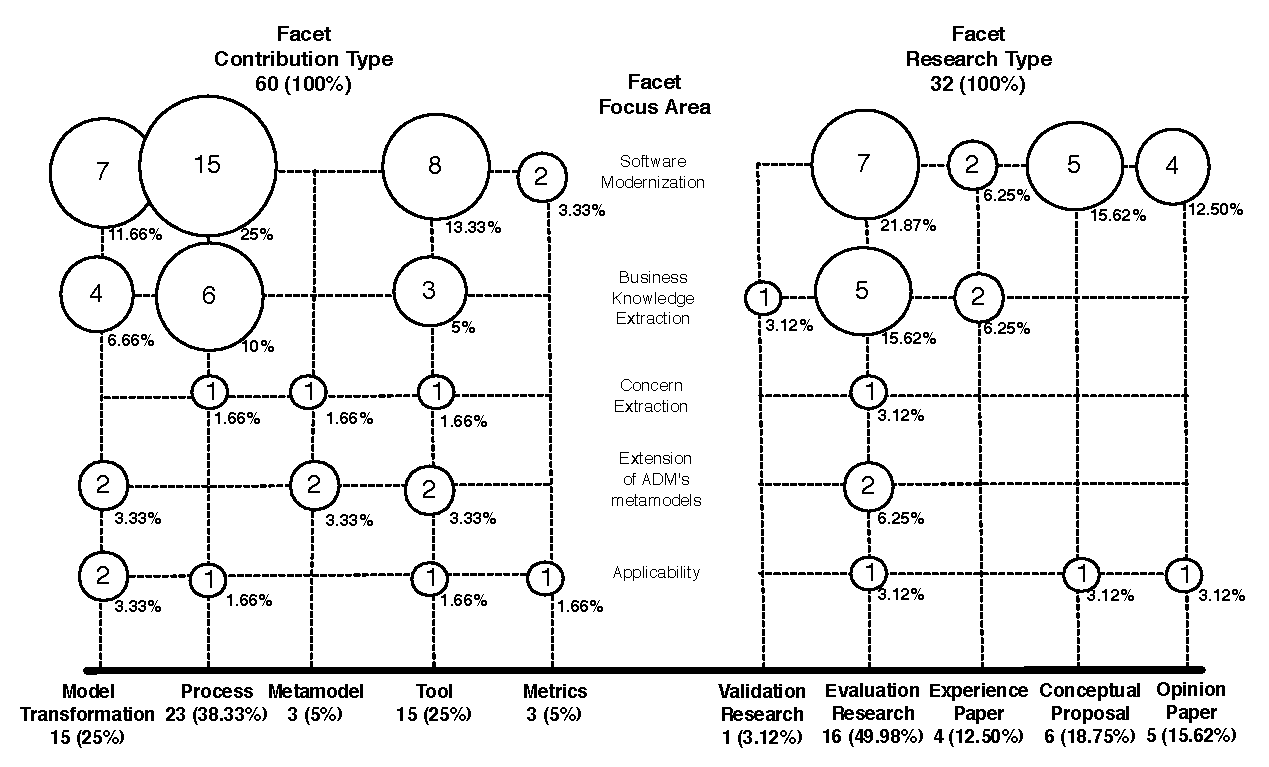
\includegraphics[scale=0.58]{figuras/Nova_Mapa2}
\caption{Map of research focus on ADM and its metamodels.}
\label{map}
\end{figure*} 

Aiming to show our results and also the frequencies of all publication related to ADM a bubble plot was plotted, which is depicted in Figure~\ref{map}. Bubble plots are essentially two x-y scatter plots with bubbles in category intersections. The size of each bubble is determined by the number of primary studies that have been classified as belonging to the categories corresponding to the bubble coordinates. This visual summary provides a bird's-eye view that enables one to pinpoint which categories have been emphasized in past research along with gaps and opportunities for future research.
%
Figure~\ref{map} has three facets: \textbf{contribution type}, \textbf{focus area} and \textbf{research type}. 
%
%In Figure~\ref{map} the facets we used for organizing the map are the \textbf{contribution type}, \textbf{focus area} and \textbf{research type}. 
%
It is worth highlighting that certain primary studies were grouped in more than one category, affecting the frequency count; i.e., the sum of the frequencies shown in each facet can be greater than the total of selected studies presented earlier (30). By observing Figure~\ref{map} can be seen that the majority of research papers are specifically dedicated for providing \textbf{Process} to assist software engineer during the modernization of legacy system to another platform/architecture. Similarly, \textbf{Model transformation} and \textbf{Tools} are also another field which have been researched. Maybe this happened once the majority of the primary studies found which describe a process, usually propose a set of model transformation and also either semi-automatic tool or a fully-automatic one. In other hand, the contribution type with less studies are \textbf{Metamodel} and \textbf{Metrics}. Thus, it is argued that primary studies that describe process to assist the modernization of legacy systems by means of ADM, papers which show a set of rules to be applied during model transformation among the ADM's metamodels (KDM, SMM and ASTM), and papers which devise tools to assist ADM's process are evidence clusters. In other words, where there may be scope for more complete literature reviews to be undertaken. Whereas metamodels (i.e., papers that explain how to extend ADM's metamodels) and metrics (i.e., papers which describe how to apply metrics in ADM's metamodel) can be regarded as gaps, thus new or better primary studies are required. 

%Summing up, \textbf{Process} to assist software engineer during the modernization of legacy system to another platform/architecture, \textbf{Model transformation} and \textbf{Tool} have been covered by over 43\%, 29\% and 17\%, respectively of the current research (see Figure~\ref{fig:bar}). On the other hand, \textbf{Metamodel} and \textbf{Metrics} have been addressed by a very small number of publications i.e., 3.92\% and 5.88\%, respectively (see Figure~\ref{fig:bar}).   %pieEvaluation


%\begin{figure*}[!h]
% 
%    \subfloat[Frequency of studies in each category.\label{fig:bar}]{
%     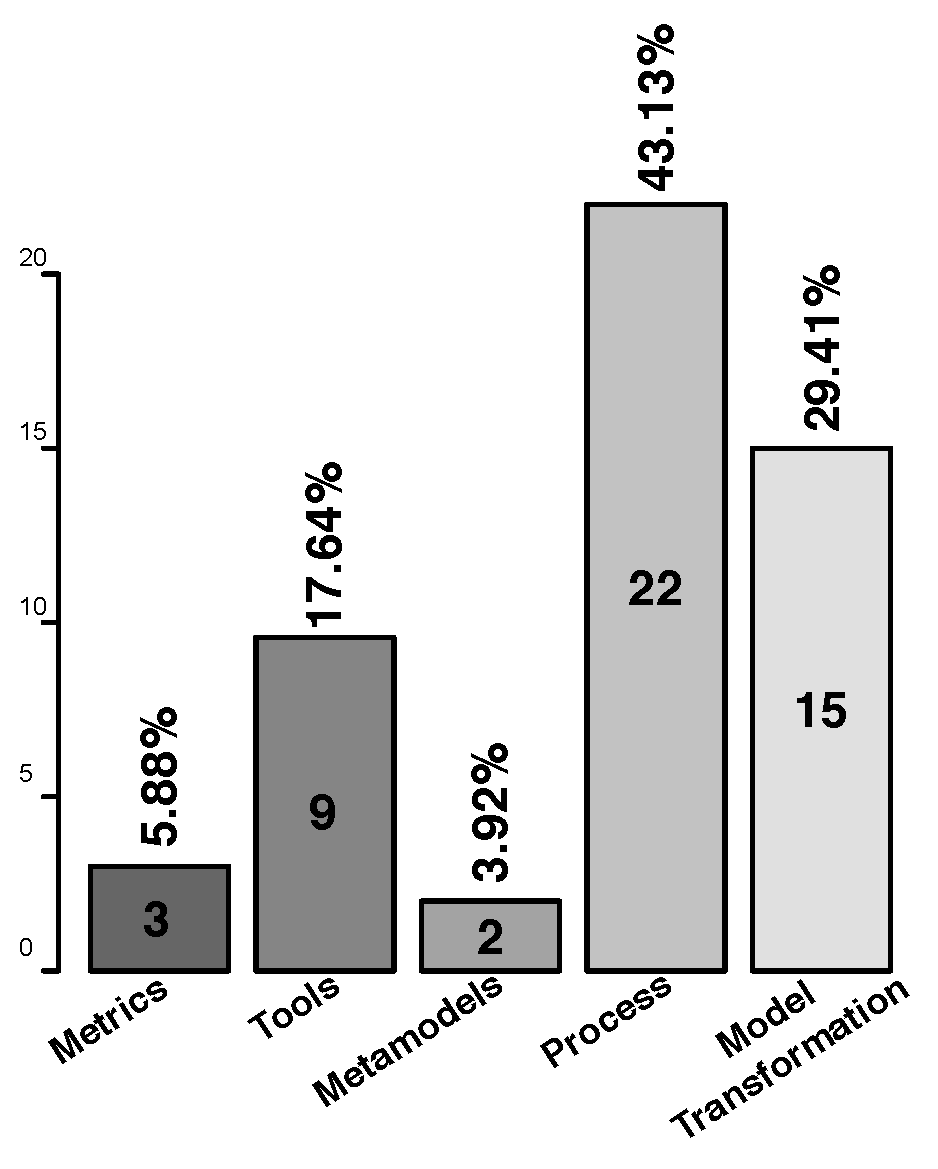
\includegraphics[width=0.2\textwidth]{figuras/NovoBarFormated}
%    }
%    \hfill
%    \subfloat[Frequency of ADM's metamodels used in literature.\label{fig:pie}]{%
%      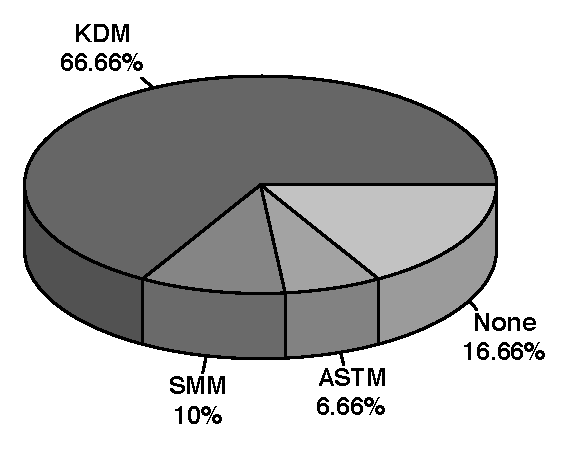
\includegraphics[width=0.2\textwidth]{figuras/pieChartModel}
%    }
%  \hfill
%    \subfloat[Frequency of research type.\label{fig:pieEvaluation}]{%
%      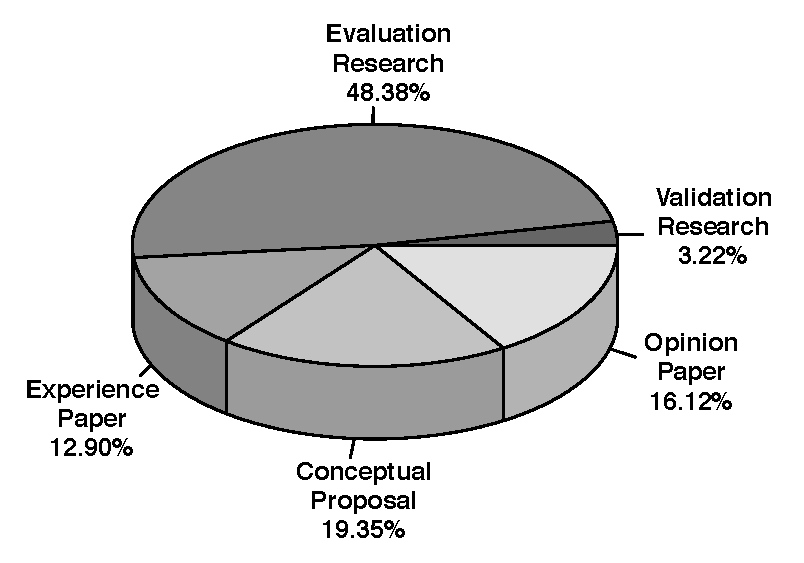
\includegraphics[width=0.25\textwidth]{figuras/pieEvaluation}
%    }
% \hfill
%    \subfloat[ADM standard metamodels used in the literature.\label{fig:pieEvaluation}]{%
%      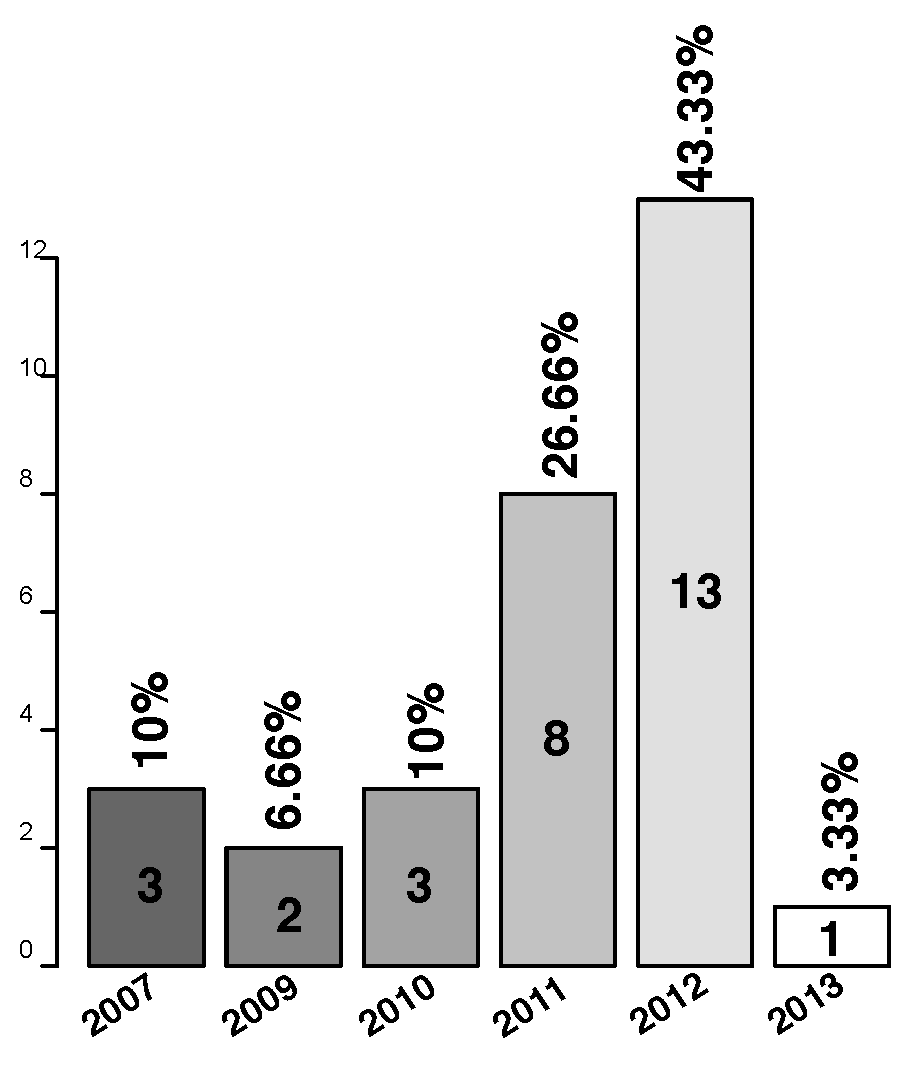
\includegraphics[width=0.2\textwidth]{figuras/DistribuicaoANoArtigos}
%    }
%    \caption{Data gathered.}
%    \label{fig:dummy}
 
% \end{figure*}

%\begin{figure}[!h]
% \centering
  % Requires \usepackage{graphicx}
%  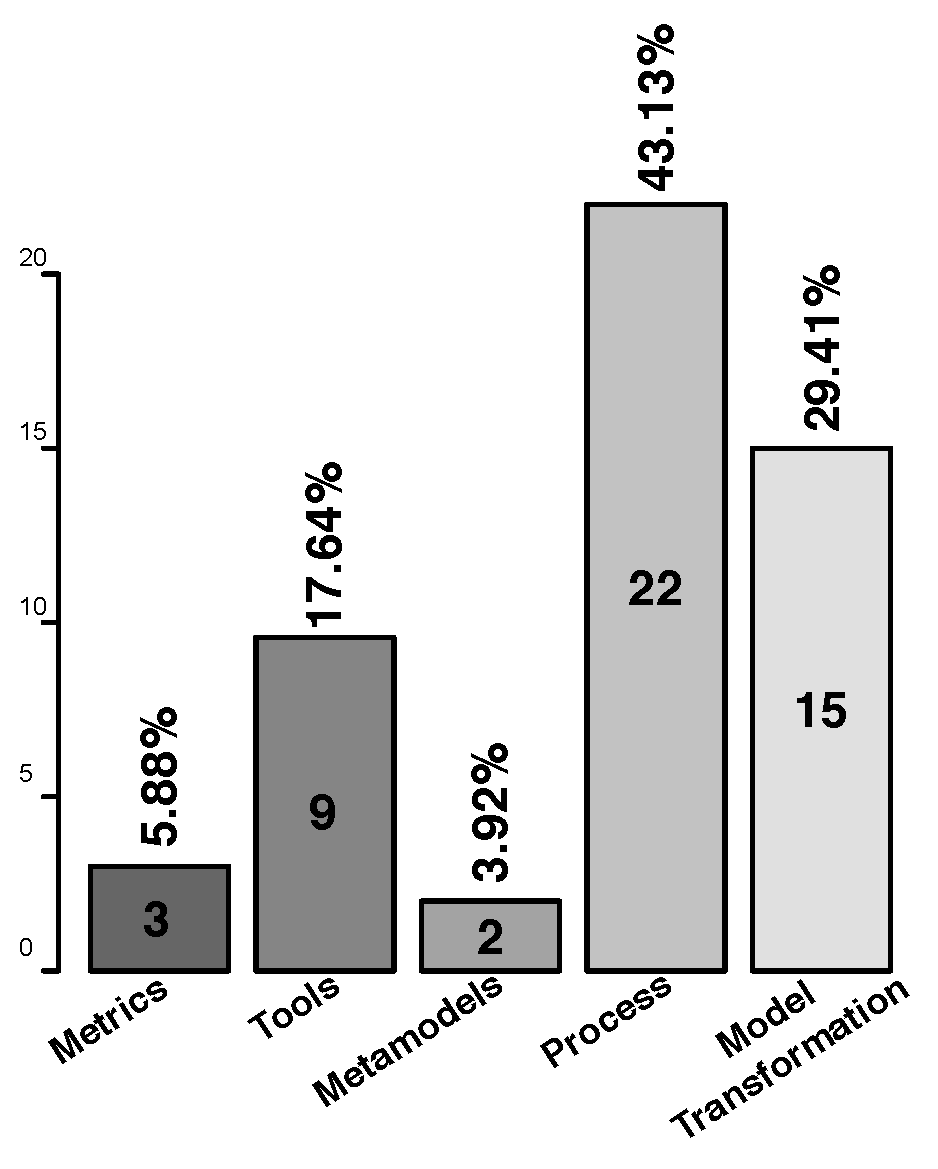
\includegraphics[scale=0.3]{figuras/NovoBarFormated}
% \caption{Frequency of studies in each category.}
% \label{fig:bar}
% \end{figure} %foi esse que eu removi, é o correto...

 As result of this analysis we answered partially the \textbf{RQ$_1$}. We answered the types of contributions that have been presented so far in literature related to ADM and its metamodels. Another part of the \textbf{RQ$_1$}, i.e., (a discussion about the focus area regarding the ADM) has been covered in the following Sections~\ref{ssub:approach} through \ref{ssub:applicability}. %Likewise, at the end of these sections we present some directions of new research that we ascertained during the review, i.e., we pinpoint some open issues that still need to be researched in ADM. 

As for answering the first part of \textbf{RQ$_2$} we analyzed all primary studies focus on gathering which ADM standard metamodels have more been used in the literature. In Figure~\ref{foo}(a) is depicted a pie chart wherein we plotted the collected data. As can be seen in this figure, KDM seems to be the metamodel which has been most used in the literature, covering over 66\%. A small percentage of primary studies have reported on the use of SMM (10\%). While ASTM has been presented by rather small percentage of 6.66\%. Finally, we found a total of 16.66\% of primary studies that does not show explicitly which metamodel has been used during the process of modernization of a legacy system. In order to answer the second part of \textbf{RQ$_2$} we gathered which are the packages most and least used within the KDM according to the identified studies. In Figure~\ref{foo}(b) it is fairly evident that the packages Code and Action are the most used in the literature (65\%). Maybe the reason for this happened are twofold: (\textit{i}) these packages are often used to represent the source-code of system and since most of the studies found use somehow the source-code as input to start the modernization process; and (\textit{ii}) the absence of a complete parser to instantiate all KDM's layers. The third one most used is the Data package (15\%). This package is used to represent relational data, such as database, XML, etc. The packages least used are Event and UI, see Figure~\ref{foo}(b). 

\begin{figure}[!h]
 \centering
  % Requires \usepackage{graphicx}
  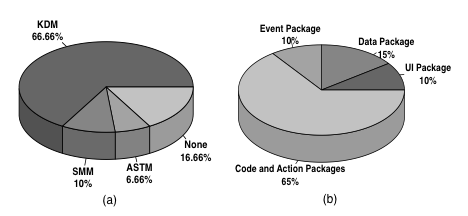
\includegraphics[scale=0.5]{figuras/todos2}
 \caption{Frequency of ADM's metamodels used in literature and packages most and least used.}
 \label{foo}
\end{figure} 


%\begin{figure}
%\def\tabularxcolumn#1{m{#1}}
%\begin{tabularx}{\linewidth}{@{}cXX@{}}
%
%\begin{tabular}{cc}
%\subfloat[\label{fig:pie}]{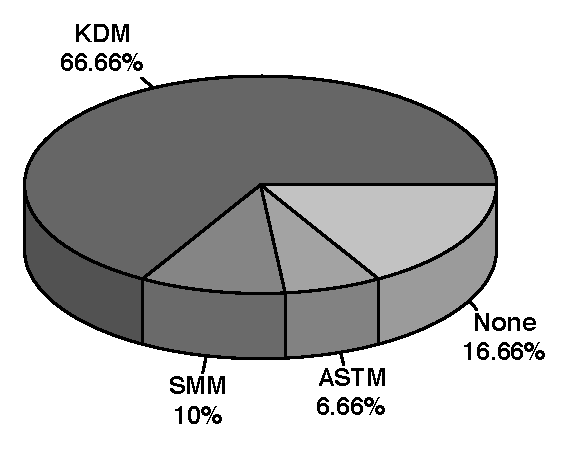
\includegraphics[width=3.9cm]{figuras/pieChartModel}} 
  % & \subfloat[\label{fig:piePackage}]{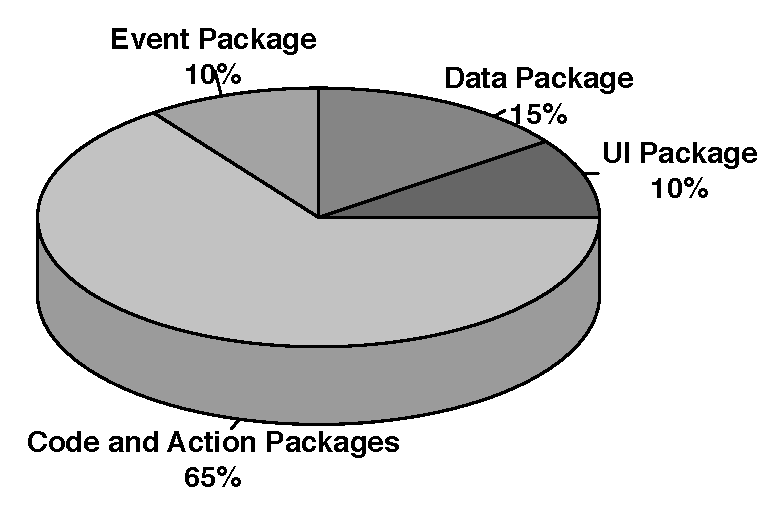
\includegraphics[width=4.5cm]{figuras/PackagesKDMFormatted}}\\
%\end{tabular}
%\end{tabularx}

%\caption{Frequency of ADM's metamodels used in literature and packages most and least used.}\label{foo}
%\end{figure}

To answer the \textbf{RQ$_3$} the data on the facet \textbf{Research Type} were analyzed, see Figure~\ref{map} on the right side.
%
%On the facet \textbf{Research Type}, shows the data we gathered related to the research type employed in the field of ADM (\textbf{RQ$_3$}). 
As far as the research type is concerned, \textbf{Evaluation Research} are in vast majority, covering 15 primary studies. A small number of publications have reported on \textbf{Validation Research} and \textbf{Experience Paper}, i.e., 1 and 4, respectively. While \textbf{Conceptual Proposal}
 and \textbf{Opinion Paper} have been presented collectively by rather of 11 primary studies.
 %Aiming to answer \textbf{RQ$_4$} we collected the name of the conference, name of the journal and the name of the workshop which the primary studies were published, Table~\ref{tab:avenue} covers the second dimension of our results and shows all avenues identified during the conducting of this review. It is fairly evident from observing the Table~\ref{tab:avenue} that the majority of primary studies were published in conference. Therefore, as result the majority of the data related to the systematic review herein were extracted from conference, i.e., among the identified primary studies (30) 23, i.e., 76.66\% studies were published in conference. Even though research has appeared on different conference we can see that in Table~\ref{tab:avenue} that we found out six journals during the review, which represent 20\%, i.e., 6 of the primary studies identified and gathered. The table also reveals that there is only one publication related to ADM and its metamodels that has appeared in a workshop so far.

 %\begin{figure}[!h]
 %\centering
  % Requires \usepackage{graphicx}
 %  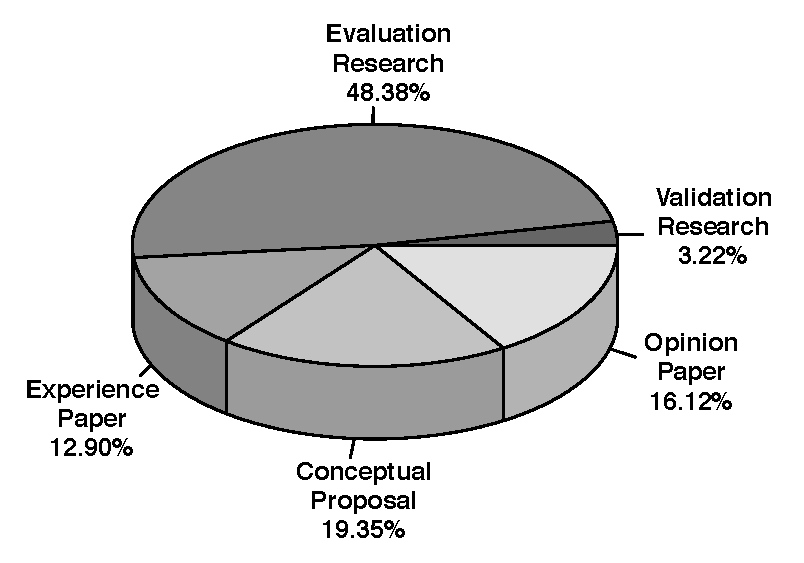
\includegraphics[scale=0.45]{figuras/pieEvaluation}
 %\caption{Frequency of research type.}
% \label{fig:pieEvaluation}
%\end{figure} 
%18 mining techniques for crosscutting concerns, as result we have answered the first part of the RQ$_1$. Based upon this bubble plot, we argue that the answer to second part of the RQ$_1$ is that Fan-In Analysis, Identifier Analysis and Dynamic Analysis are the techniques most used and Program Analysis Based, XScan-Concern-Peers, Data-Flow and Model Driven are the least used. More precisely, among the 62 primary studies included herein, 27 describe Fan-In Analysis, Identifier Analysis or Dynamic Analysis, respectively. In other hands, the techniques with less studies available in literature are Program Analysis Based, XScan-Concern-Peers, Data-Flow and Model Driven. Furthermore, it is argued that Fan-In Analysis, Identifier Analysis and Dynamic Analysis are evidence clusters (i.e., where there may be scope for more complete literature reviews to be undertaken). In contrast, Program Analysis Based, XScan-Concern-Peers, Data-Flow and Model Driven can be deemed as ``evidence desert'' (i.e., wherein better or new research is required). 

%Finally, in Figure~\ref{fig:distribuicao_de_artigo_por_ano} shows the distribution by year of the accepted primary studies. As can be seen, the year 2012 had the biggest number of publications related to ADM and its metamodels, i.e., 43.33\%. Among the 30 primary studies included herein 8 were published in 2011, i.e., 26.66\%. In 2007 and in 2010 were published 3 primary studies related to ADM and its metamodels, representing 20\% of all primary studies. Among the 30 primary studies any of them were published in 2008. In 2009 was identified a percentage of 6.66 of primary studies related to the review herein. Taking into account the search strings was applied in 2013, it may explain the low amount of primary studies published in 2013. 

 %\begin{figure}[!h]
 %\centering
  % Requires \usepackage{graphicx}
  % 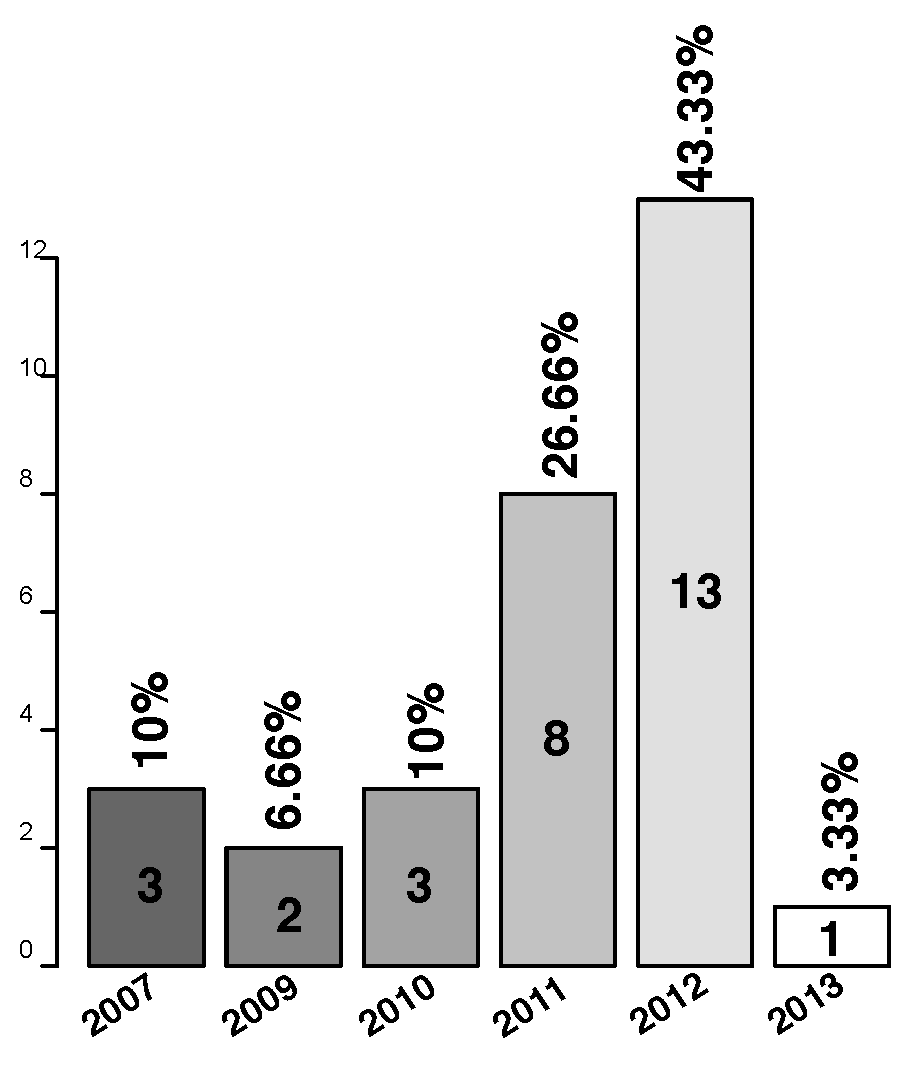
\includegraphics[scale=0.35]{figuras/DistribuicaoANoArtigos}
 %\caption{Distribution of publication by years.}
% \label{fig:distribuicao_de_artigo_por_ano}
%\end{figure} % esse é o correto 

%As depicted in second bar of the Figure~\ref{fig:bar}, we identified 9 tools. Among them six were developed to assist the modernization of legacy systems. The remainder were elaborated to transform the legacy sytem's source-code into instance of ADM's metamodels. In Table~\ref{tab:tools} has four columns to categorize, name and reference such tools. The column, Cat., stand for ``Categories'' of the tools. There are two categories: (\textit{i}) \textbf{Modernization} which represents tool that assist to modernize legacy systems to another platform/architecture, and (\textit{ii}) \textbf{Abst.} (``Abstraction'') which symbolises tool that takes the legacy system's source-code and instantiate a representation of the ADM's metamodels, i.e., brings the source-code into another abstraction level. By using this table was possible to  answer the first part of the \textbf{RQ$_5$}. As for answering the second part of it, a brief description about the identified tools are presented as follows. 

%\begin{table}
%\scriptsize
%\centering
%\caption{The analyzed information of each tool.}
 % \begin{tabular}{|>{\centering}p{0.6cm}|l|l|l|}
%\hline 
% \cellcolor{gray} Cat. & \cellcolor{gray}Name & \cellcolor{gray}Ref & \cellcolor{gray}Website\tabularnewline
%\hline 
%\hline
%\multirow{6}{*}{\begin{sideways} 
%Modernize
%\end{sideways}} &
%CloudMIG &\cite{SMR:SMR582}  & tinyurl.com/cloudmigxpress\tabularnewline
%\cline{2-4}  
%& MARBLE &\cite{Perez-Castillo:2011:ECS:1982185.1982249,6080834, 6498507,Perez-Castillo:2010:IBP:1875847.1875861}  & No\tabularnewline
%\cline{2-4} 
%& MIMOS &~\cite{6498507} & No\tabularnewline
%\cline{2-4} 
%& PRECISO &~\cite{delCastillo:2009:PRP:1529282.1529753}  & No\tabularnewline
%\cline{2-4} 
%& R2SOA &~\cite{Guzman:2007:AAR:1339262.1339532} & No\tabularnewline
%\cline{2-4} 
%& WA2RIA &~\cite{Rodriguez-Echeverria:2011:MLW:2186508.2186536}  & No\tabularnewline
%\hline
%\multirow{3}{*}{\begin{sideways} 
%Abst.
%\end{sideways}} 
%& COMO &\cite{5773392}  & No\tabularnewline
%\cline{2-4}  
%& Gra2MoL &\cite{5440163}  & modelum.es/trac/gra2mol/\tabularnewline
%\cline{2-4}  
%& MoDisco &~\cite{Bruneliere:2010:MGE:1858996.1859032} & eclipse.org/MoDisco/\tabularnewline
%\hline 
%\end{tabular}
%\label{tab:tools}
%\end{table}

%\textbf{CloudMIG} provides a semi-automatically support for the migration of software systems to PaaS or IaaS-based clouds by using KDM. This tools identifies the possible services by applying a set of rules heuristics., such as: Distribute the five most frequently used services to own virtual machines or the server methods responsible for at least 10\% of overall consumption of the CPU time shall be moved to client side components if they do not need access to the database. After, CloudMIG can generate considerable parts of a resource-efficient target architecture utilizing these rules heuristics~\cite{SMR:SMR582}. 


%\textbf{MARBLE} is a modernization tool to recover business processes from legacy systems based on KDM. It uses two process mining techniques, static and dynamic analysis of source code to identify business processes. The static one is based on a module that analyze the source code file (Java files in particular) and builds an abstract syntax tree of the source code and then create an instance of KDM. On the other hand, the dynamic one takes the information about the system execution into account to extract meaningful business knowledge.

%\textbf{MIMOS} is a tool to recover business processes from legacy systems based on KDM~\cite{6498507}. This tool uses parser to identify the business processes, then a set of refactoring techniques is applied to KDM.

%\textbf{PRECISO} is a tool for database modernisation through Web Services. Potential services can be simultaneously discovered along with database reverse engineering. A set of patterns are sought in recovered database schema~\cite{delCastillo:2009:PRP:1529282.1529753}.

%\textbf{R2SOA} is a complete process to reengineer relational databases at a model level to integrate them into SOA contexts as a set of services. Firstly, database schema is reversed and a suitable model is built from the metadata extracted from the database catalog. Based on the structure of the database schema, a first service extraction can be undertaken, a set of model driven pattern matching is used, then CRUD operations are automatically included~\cite{Guzman:2007:AAR:1339262.1339532}.

%\textbf{WA2RIA} can modernize legacy Web Applications (WA) to Rich Internet Applications (RIAs) by using ADM and KDM. This tool uses MoDisco to get an instance of KDM, then a set of rules are applied to realize the modernization of the WA to RIA~\cite{Rodriguez-Echeverria:2011:MLW:2186508.2186536}.

%\textbf{COMO} provides an extension to KDM with the concepts of component and interface. By lifting the abstraction level, COMO can produce an adequate view of the entire system, and leverage the boundaries between components to better focus the subsequent modernization effort~\cite{5773392}. This tool neither offer a semi-automatically or automatically way to identify the components, i.e., the engineer has to identify the components. \textbf{Gra2MoL} has been specifically designed to address the problem of extracting models from source code. Gra2MoL is a rule-based transformation language like existing model-to-model transformation languages, but with the fundamental difference that the source element of a rule is a grammar element instead of a source metamodel element~\cite{5440163}. Gra2MoL uses parsers to identify and to extract models from source code. \textbf{MoDisco} aids to offer an open source generic and extensible MDD framework. It aims at providing the required capabilities for creating models and allowing there handling, analysis and computation~\cite{Bruneliere:2010:MGE:1858996.1859032}.

\section{A brief discussion on the focus areas identified within ADM}

Here we organized each subsection in a way to describe the focus areas identified in this systematic review.

\subsection{Approach to modernize legacy systems to another platform/architecture} % (fold)
\label{ssub:approach}

 Jorge Maratalla et al., propose \textbf{GAFEMO}~\cite{6311013} which aims to modernize a legacy systems to service-oriented approach taking advantage of the features provided by gap-analysis techniques. This approach takes as input a legacy system and then creates KDM representation of it. After, a set of rules are applied in this model to create the services. In~\cite{6080786} the authors present a method that combines ADM with program analysis techniques to support analysis across the components of a component-based system. They builds upon the foundations laid out by OMG's KDM to reverse engineer a homogeneous system-wide dependence model from a software system's heterogeneous source and configuration artifacts, and use this model as the basis for the analysis. In~\cite{Mazon:2007:MDM:1784489.1784497} the authors propose a modernization approach for the modernization of Data warehouses following the concepts of ADM. The approach automatically performs the following tasks: (\textit{i}) obtain a logical representation of data sources (\textit{ii}) mark this logical representation with MD concepts, and (\textit{iii}) derive a conceptual MD model from the marked model. In~\cite{Guzman:2007:AAR:1339262.1339532} is defined an approach which is focused on the analysis of legacy systems to discover and create functionalities to be exposed as services using Web Services. It is based in five steps: (\textit{i}) Database reverse engineering: database schema is reversed and a suitable model is built; (\textit{ii}) First service extraction: based on the structure of the database schema, a first service extraction can be undertaken; (\textit{iii}) PIM generation: is obtained from the PSM representation using a model-to-model transformation, CRUD operations are automatically created; (\textit{iv}) Service discovering: abstract objects are identified in the PIM; (\textit{v}) WSDL (Web Service Description Language) generation: using the PIM, a model-to-model transformation and a WSDL  metamodel are generated to expose the services discovered and created in the PIM and the PSM. 

In~\cite{5741334, SMR:SMR582} is proposed an approach based on ADM named CloudMIG that aims at supporting SaaS (Software as a Service) providers to semi-automatically migrate legacy software systems to the cloud. It is composed of six major steps: (\textit{i}) Extraction: Includes the extraction of architectural and utilization models of the legacy system, the approach uses KDM; (\textit{ii}) Selection: Select an appropriate CEM- compatible cloud profile candidate; (\textit{iii}) Generation: Produces the target architecture and a mapping model; (\textit{iv}) Adaptation: The adaptation activity enables a reengineer to manually adjust the target architecture; (\textit{v}) Evaluation: Realize static analyses and a runtime simulation of the target architecture; (\textit{vi}) Transformation: The actual transformation of the existing system from the generated target architecture to the aimed cloud environment. In~\cite{4400179} the authors propose an approach that uses ADM which is focused on the analysis of legacy systems to discover and create functionalities to be exposed as services using Web Services.

 P\'{e}rez-Castillo et al.,~\cite{5328801, delCastillo:2009:PRP:1529282.1529753, ICEISPerez:CastilloGCP12} present an approach to modernize legacy systems together with the legacy relational database. This approach recovers the code-to-data linkages and obtains three kinds of models according to the ADM approach: (\textit{i}) The KDM Code Model, which represents the inventory of legacy source code. It has also the points that link the SQL Sentence Models and Database Schema Models. (\textit{ii}) The SQL Sentence Model for modeling a certain SQL query that was embedded in legacy source code. (\textit{iii}) The Database Schema Model, which represents the specific database fragment derived by an SQL Sentence Model. In~\cite{FuentesFernandez2012247} presents the XIRUP modernization methodology, which proposes a highly iterative process, structured into four phases: preliminary evaluation, understanding, building and migration. This modernization process is feature-driven, component-based, focused on the early elicitation of key information, and relies on a ADM.

%Mainetti et al.,~\cite{Mainetti:2012:MMT:2364120.2364182} present an approach that allows developers to automatically modernize the client side of legacy systems. In this approach developers can refactor the Graphical User Interface (GUI) of legacy systems during the modernization, taking the opportunities offered by novel interaction paradigms, i.e., Rich Internet Application (RIA). 

In~\cite{Rodriguez-Echeverria:2011:MLW:2186508.2186536} the authors present an approach for the definition of a systematic process for Web Applications (WA) to RIA modernization, by applying ADM principles. The approach presented by the authors consists on generating a RIA client from the legacy WA presentation and navigation layers and its corresponding service-oriented connection layer with the underlying business logic at server side. Boussaidi et al.,~\cite{6385130} propose an approach that makes use of the KDM to reconstruct and document software architectural views of the legacy system. They consider an architectural view to be a way of partitioning a system using a specific set of KDM relevant concepts and relations and they propose clustering algorithms that target specific views mainly a layered view that we call horizontal view and a feature based view that we call vertical view. In~\cite{5440163} ADM is used into practice by building a modernization tool to generate metric reports of legacy Oracle Forms applications to assess migration efforts. The authors devised an extractor that generates KDM models from PL-SQL code (PL/SQL-to-KDM) and a metrics report generator for these KDM models. 

\subsection{Business Knowledge Extraction}
\label{ssub:Business_Knowledge_Extraction}

 P\'{e}rez-Castillo et al.,~\cite{Perez-Castillo:2011:ECS:1982185.1982249,6080834, 6498507,Perez-Castillo:2010:IBP:1875847.1875861} present an approach to recover business processes from legacy systems. This approach is based on a set of transformation: (\textit{i}) transformation obtains PSM models from each legacy software artifact using a specific metamodel for each artifact; the traditional reverse engineering techniques such as static analysis, dynamic analysis, and formal concept analysis and so on, can be used to extract the needed knowledge; (\textit{ii}) a set of model transformations to obtain a KDM model built from the PSM models at (\textit{i}); (\textit{iii}) a transformation finally obtains the current business process model, this transformation is based on a set of business patterns. In~\cite{PerezCastillo20121370} the authors report the results of a family of case studies that were performed to empirically validate this approach. %P\'{e}rez-Castillo et al., also provides in~\cite{} a semi-automatic technique based on dynamic analysis, combined with static analysis to instrument the source code for obtaining event log models. A set of model transformation to transform the event log into another model following the KDM to depict legacy system, concerning its runtime viewpoint, which can be used in any software modernisation project. In~\cite{Perez-Castillo:2010:IBP:1875847.1875861} P\'{e}rez-Castillo et al., explain the KDM2BPMN model transformation within MARBLE, an ADM-based framework to rebuilt business processes embedded in legacy systems in order to facilitate and improve the evolutionary maintenance.

Normantas and Vasilecas ~\cite{lastDAyOFMyLife} present an approach that facilitates software comprehension by enabling traceability of business rules and business scenarios in software system, i.e., their approach aim to extract business specific knowledge from the knowledge about the existing software system represented within the KDM. Ropero et al.,~\cite{Fernandez-Ropero:2012:EAB:2367051.2367064} describes a set of rules to transform Mining XML (MXML) metamodel, which is common used to represent the sequence of business activities executed by an enterprise system to KDM. %The authors takes an MXML model and obtains an equivalent KDM model at the same abstraction level. The proposed set of rules consist of eight declarative transformation rules. 


\subsection{Extension of ADM's metamodels} % (fold)
\label{ssub:extension_of_adm_s_metamodels}

%We identified three papers that address how to perform extension of ADM's metamodels. We provided a brief summary of these paper are follows.

In~\cite{5773392} the authors propose the COMO (Component-Oriented MOdernization) metamodel an KDM's extension, by borrowing recurring concepts from component-based solutions and software architectures, and to support a proper componentization of the system to assist the modernization of legacy systems. In~\cite{Perez-Castillo:2012:IEL:2231936.2231949} propose an extension to the KDM that aims to represent all the information registered in a MXML model in the KDM model. In~\cite{library7329} the author proposes an extension of the KDM to represent all elements of the Aspect Oriented Paradigm, i.e., aspect, advice, point-cut, can be represented using the KDM. All these three paper have in common is that the authors claimed the impact of these extensions on well-proven and KDM based tools is not problematic since they are performed with the own extension mechanism of the KDM standard.

% subsubsection extension_of_adm_s_metamodels (end)

\subsection{Applicability} % (fold)
\label{ssub:applicability}

%We also identified a small number of papers that address just the applicability of the ADM and its metamodel. 

P\'{e}rez-Castillo et al.,~\cite{PrezCastillo2011519, Perez-Castillo:2012:IEL:2231936.2231949, 6498507} present how to apply KDM to modernize legacy systems. Also, the authors described each layer of the metamodel KDM, they also presented a set of example of how to use ADM and KDM during the modernization of a legacy systems. The authors claim that the paper enables researchers and practitioners to get a better understanding KDM

% subsubsection applicability (end)










\section{Discussion}\label{sec:discussion_and_threats}
	Herein is provided a summary of key findings of this review. Also, here is pinpointed some open issues that still need to be researched in ADM.

\subsection{Main Findings}\label{sec:principle_findings}
	Recent proposals in ADM have focused mainly on providing approaches to modernize legacy system to another platform/architecture resulting in appearance of several proposals, see Section~\ref{ssub:approach}. However, if we look at overall problem of the integration of modernization into an ADM context, there is still a significant work to be done. Following the ADM approach, models are the main focus for visualizing an executable view of the system and are also used to modernize a system. Therefore, in order to integrate ADM's metamodels into this larger context, the area of discovering knowledge, i.e., parsers, needs more attention along with solution to verification of models. Very few works have been reported on in the literature (e.g.,~\cite{5440163,Bruneliere:2010:MGE:1858996.1859032}) so far that have addressed parsers to represent instances of KDM, but even these parsers provide limited infrastructure to represent all KDM's layers. Thus, new researches must be conducted to create a complete parser in order to represent all KDM's layer. Besides, the discovering of knowledge are often mostly static in a sense that they are unable to obtain knowledge during the executing of the target legacy system. In~\cite{5871783} the authors presented an approach that dynamically discovery knowledge of the target system during its execution. Nevertheless, this approach lacks support for complex discovery of knowledge once it is just based on the KDM's event metamodel package. Hence further research is required to boost the discovering of knowledge, e.g., use the knowledge dynamically identified combined with other models of KDM as the code and data models in order to acquire more meaningful models, since these models make it possible to consider additional sources of embedded knowledge.

In addition, we observed that there are three main hurdles in need to be more researched so that modernization techniques can be used in the ADM approach in an effective and widespread way. The first hurdle is the present lack of a fully developed idea of ``good'' KDM style. This is an important issue, for a clear notion of style is a fundamental prerequisite for the use of modernization, enabling software engineers to see where they are heading when modernizing their legacy system with KDM. Fowler et al.~\cite{refactImpro} advocated a specific notion of style for Object-Oriented Programming (OOP) through a catalog of 22 code smells, compounded by a catalog of 72 refactorings through which those smells can be removed from existing code. A second one - both a cause and a consequence of the first - is the present lack of a KDM equivalent of such catalogues. We assume that the process of modernization by using KDM would equally benefit from KDM specific catalogues of smells and refactorings, helping software engineers to detect situations where the KDM could be improved and guiding them through the corresponding transformation processes. A third hurdle is the absence of tool that supporting refactoring by using the KDM specification in current integrated development environments. The catalogue presented by Fowler et al.~\cite{refactImpro} provided a basis on which developers could rely to build tool support for object-oriented refactoring: similar catalogue for the KDM specification are likely to bring similar benefits to assist software engineers during the modernization process.

\subsection{Threats to Validity}\label{threats}
		%The main threats to validity identified in the review are described next:

\textbf{Primary studies selection}: Aiming at ensuring an unbiased selection process, we defined research questions in advance and devised inclusion and exclusion criteria we believe are detailed enough to provide an assessment of how the final set of primary studies was obtained. However, we cannot rule out threats from a quality assessment perspective, we simply selected studies without assigning any scores. In addition, we wanted to be as inclusive as possible, thus no limits were placed on date of publication and we avoided imposing many restrictions on primary study selection since we wanted a broad overview of the research area. \textbf{Missing important primary studies}: We conducted the review in several search engines, even though it is rather possible we missed some primary studies. We mitigated this threat by selecting search engines which have been regarded as the most relevant scientific sources~\cite{Kitchenham}. \textbf{Reviewers reliability}: The reviewers of this study are researchers in the software reuse field. So, we are not aware of any bias we may have introduced during the analyses. \textbf{Data extraction}: Another threat for this review refers to how the data were extracted from the digital libraries, since not all the information was obvious to answer the questions and some data had to be interpreted. In order to ensure the validity, multiple sources of data were analyzed, i.e. papers, technical reports, white papers. In the event of a disagreement between the two primary reviewers, a third reviewer acted as an arbitrator to ensure full agreement was reached.


\section{Concluding Remarks}\label{conclusion}
		Our long-term research goal is to find out how ADM has been applied in the literature to assist software engineers during the process of modernization of legacy system. To do so in this paper we presented a systematic review of ADM and its metamodels, following the process described by Kitchenham~\cite{Kitchenham}. Through an examination of 30 primary studies, this review has presented 22 papers which describe processes, 15 that propose a set of model transformation, 9 that present tools, 3 which present metrics and 2 that illustrate extension in the ADM's metamodels. Notice that certain primary studies were grouped in more than one category, affecting the frequency count; i.e., the sum of the frequencies shown in each facet of the Figure~\ref{map} can be greater than the total of selected studies identified, i.e., 30. %The review described in this paper reveals that the most mentioned mining techniques for crosscutting concern are Fan-In Analysis, Identifier Analysis and Dynamic Analysis. In contrast, Program Analysis Based, XScan-Concern-Peers, Data-Flow and Model Driven can be deemed as  ``evidence desert''. 

%The initial significant contributions to ADM were presented in 2007 (i.e.,~\cite{Mazon:2007:MDM:1784489.1784497, Guzman:2007:AAR:1339262.1339532, 4400179}), in 2008 had no publications. However, in 2009 we identified two paper dealing with ADM (i.e.,~\cite{delCastillo:2009:PRP:1529282.1529753, 5328801}). Next, we had a rise from 2010 (3 papers) to 2011 (8 papers). After, in 2012  
%the rate of papers gradually rose to 13. Then, it dropped out in 2013. This may happened once we carried out the review in 2013. Among these paper were found that most of them have appeared in conferences and journal, while just a was reported in workshop. We claim that researchers can use this review as a basis for advancing the field, while practitioners can use it to identify process, tools, metrics, that are well-suited to their needs. This systematic review should serve not only academic researchers but also industrial professionals, aiming at adopting some process, tool, metrics, to modernize a legacy systems within their organizations.

In summary, this review shows that there are some researchers investigating ADM and its metamodels. As consequence, we were able to identify that there are a set of processes which have been commonly used in literature to assist the software engineer to modernize legacy system by means of ADM. Afterwards, it was also possible to identify that KDM is the ADM's metamodel more utilized in the literature. Similarly, the KDM's packages most used in the literature are Code and Action - the least used are Event and UI packages. The main future directions that emerged from this review are highlighted in Section~\ref{sec:principle_findings}. Likewise, as long term future work, related systematic reviews are about to be concluded and the relationship among their results should be investigated aiming to characterize this area in a deeper way. As soon as they are concluded, their results should be presented for the academic community as a technical report that will become available online.




%As future works, other related systematic reviews are about to be concluded and the relationship among their results should be investigated aiming to characterize this area in a deeper way. As soon as they are concluded, their results should be presented for the academic community as a technical report that will become available online.





%Research in the area of aspect-oriented modeling and model- driven code generation can result in significant advancement in development of software systems that are more maintainable, extensible and reusable. To get an overall view of the current re- search in this area, we defined a few research questions and launched a systematic mapping study. We found 65 publications that possess maximum relevance to fulfill objectives of our study. The selected papers have appeared between 2002 and 2011.
%The results of this study indicate that aspect-oriented modeling and code generation is a rather underdeveloped area. The initial significant contributions to this area were presented in 2002 (i.e. [55,56]), most papers have appeared in workshops and confer- ences, while a few were reported in journals.



%Based on the identified techniques we have extended the taxonomy proposed by Kellens et al.~\cite{Kellens}. This new taxonomy contains 7 new  mining techniques for crosscutting concerns. By using this taxonomy we hold that this taxonomy could serve as an initial roadmap to crosscutting concern researchers. Moreover, this extended taxonomy could be relevant for tool developers who might have knowledge about the best aspect indicators to use or who may have certain demands about the granularity of the results.

%The main future directions that emerged from this review are the need for empirical, comparative evaluations and the opportunity for developing combined techniques. Indeed, since every technique relies on different assumptions and uses different underlying analysis techniques, the found techniques are highly complementary, which suggests the possibility of several useful combinations. Thus, through the results obtained in this review we argue that if one pretends to devise a new mining techniques for crosscutting concerns to mine either Persistence or Observer, a good initial point is to take into consideration the combination herein illustrated in Table~\ref{table_conclusion} and~\ref{table_conclusion2} but more studies are needed because the combinations proposed did not take into consideration the versions of the system, so we intend to analyze this in future works.


% that could improve precision and recall metrics.Thus, if new mining techniques are developed then software engineers must test a wide range of concerns taking into account implementation variabilities. Finally, through the results obtained in this review we argue that if one pretends to devise a new mining techniques for crosscutting concerns to mine either Persistence or Observer, a good initial point is to take into consideration the combination herein illustrated in Table~\ref{table_conclusion} and~\ref{table_conclusion2}.


%We learned from this review that it is important to perform studies showing the pros and cons of using combinations of several mining techniques for crosscutting concern in a unique software environment. One type of analysis that can be performed is to combine techniques with high values of recall and high values of precision. Although the Table~\ref{table_conclusion} shows one tool (CBFA) using combined techniques, we can not  infer whether or not the tool has improved their capability to identify crosscutting concerns because we do not have the precision and recall metrics for each tool acting separately with the same conditions and one example is not representative. However, it could be a strategy for searching new techniques, i.e., combining CBFA with XScan. The idea behind this type of combination is to mitigate deficiencies in the way they do the identification of concerns because most probably one group of techniques is better adapted to find out a sort of concerns while others may have better results on others. Furthermore, it could be interesting to try to classify techniques according to the domain in which they act, i.e., non-functional and functional concerns. The Dynamo tool has a good precision for Persistence concern but not so good for Undo. Similarly, CBFA has a high value of precision for Undo and low value of precision for Persistence. Nevertheless, more studies are needed to confirm if Dynamo is most suitable for non-functional concern and future research might resolved this issue. We have presented candidate combinations of techniques that could improve precision and recall metrics. The comparison allowed us to show that the precision and recall can change quite a lot, when concern is different. Thus, if new mining techniques are developed then software engineers must test a wide range of concerns taking into account implementation variabilities. Finally, through the results obtained in this review we argue that if one pretends to devise a new mining techniques for crosscutting concerns to mine either Persistence or Observer, a good initial point is to take into consideration the combination herein illustrated in Table~\ref{table_conclusion} and~\ref{table_conclusion2}.

%\section*{Acknowledgments}\label{sec:Acknowledgments}

%Authors would like to thank YYYYY.

\bibliographystyle{splncs}
\bibliography{acmSac2013}
\end{document}